
\renewcommand*\descriptionlabel[1]{\hspace\leftmargin$#1$}
\setcounter{tocdepth}{5}
\setcounter{secnumdepth}{5}
\newcommand{\minus}{\scalebox{0.65}[1.0]{$-$}}

\section{Energy}

In modern society, scientific advancements and technological developments have improved quality of life drastically over time.
These commonly used technologies, such as air conditioning or food production, require an energy input in order to function properly.
%Within these advancing technologies, ranging from air conditioning to food production, there is a common thread of energy requirement.
To cool the air, energy is required in order to compress, pressurize, and cool the refrigerant. To produce food, energy is required to pump water, create fertilizer, and operate heavy machinery.
Energy, typically in the form of electricity, is significant in maintaining and developing quality of life for society.

However, energy is not free, and it takes effort to harvest and convert energy into usable forms. For wind power, this means building large turbines which can be turned by the wind. For solar power, this means building solar panels, which convert photons from the sun into electrical energy. However, for most large-scale electrical generation needs, it is more efficient for the conversion aspect to use boiling water to turn a turbine, which then generates electricity, as can be seen in Figure \ref{fig:energy-gen-methods}. The methods shown which use boiling water account for over 75\% of the total energy generation in the United States.
%Regardless of how it is generated, electricity can then be transported or stored to be used by people for any variety of purpose. 

\begin{figure}[H]
  \centering
  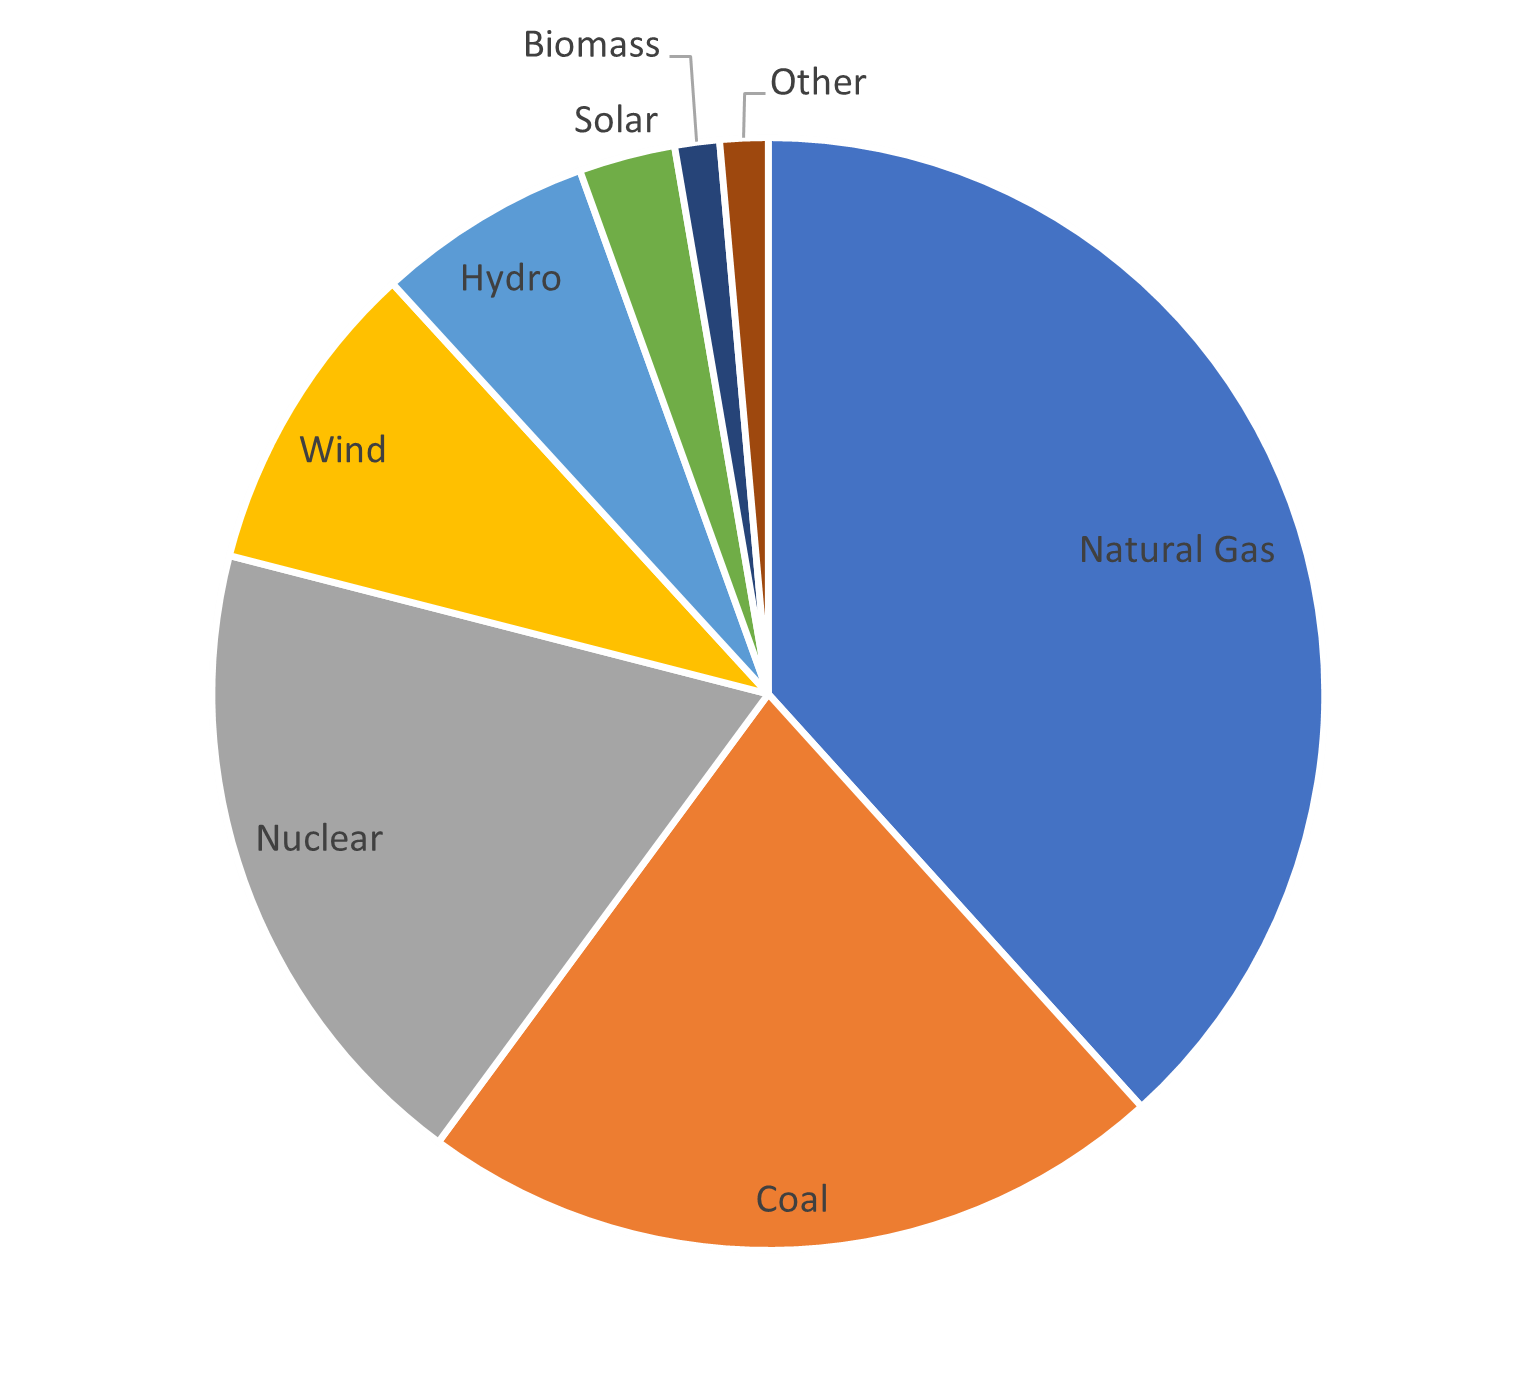
\includegraphics[scale=0.7]{images/US-energy-prod.png}
	\caption{Energy generation in the United States in 2021 from the US Energy Information Administration \cite{tyra_electric_2022}.}
   \label{fig:energy-gen-methods}
\end{figure}

Figure \ref{fig:energy-gen-methods} shows the different methods of energy generation in the United States. From this figure, it can be seen that the methods which dominate energy contribution are natural gas, coal, and nuclear.
Of the various methods to generate electricity, desirable characteristics are safety, efficiency, consistency, availability, and economics.
Nuclear energy contains several of these characteristics: safety can be seen in Table \ref{tab:death-mega}, thermal efficiency from the high temperatures which are generated, and consistency by providing a constant supply of energy except during scheduled outages.
Nuclear energy has many positives, though there is an economic problem due to high up-front costs, which are on the order of \$10 billion for a 1GW nuclear power plant \cite{du_update_2009}. Additionally, availability is lowered due to issues such as siting, public perception, and construction issues. 

\section{Nuclear Energy}

Part of the reason nuclear energy has high up-front costs is because the nuclear industry is highly safety conscious and has many regulations in place in order to minimize risks.
Although this mindset increases costs, the effort has paid dividends, which can be seen in Table \ref{tab:death-mega}. This table shows mortality rate normalized to energy produced and shows that nuclear energy is one of the safest energy sources available.
%Although this mindset increases costs, the effort has paid dividends, which is apparent when viewing the deaths associated with different energy generation methods, shown in Table \ref{tab:death-mega} \cite{brook_why_2014}.

\begin{table}[H]
\renewcommand{\arraystretch}{1.25}
\caption{Mortality rates for each energy source in deaths per billion kWh produced (recreated from \cite{brook_why_2014}).}
\label{tab:death-mega}
\begin{center}
\begin{tabular}{ | c | c | }
 \hline
 Energy Source & Mortality Rate (deaths per billion kWh)\\
 \hline
 \hline
 Coal (Global Average) & 100 \\
 Biofuel/Biomass & 24 \\
 Coal (U.S.) & 15 \\
 Oil & 36 \\
 Natural Gas & 4 \\
 Hydro (Global Average) & 1.4 \\
 Solar (Rooftop) & 0.44 \\
 Wind & 0.15 \\
 Nuclear (Global Average) & 0.04 \\
 
 \hline
\end{tabular}
\end{center}
\end{table}

Even though the up-front costs are high, nuclear plants are a long term investment. Nuclear power plants are licensed to operate for 40 years and can get extensions to extend that time by 10-20 years \cite{bredimas_international_2008}.
%This means that nuclear plants are a very long term investment.
An investment at this time scale is difficult to make for a private industry though, as there is less risk when investing in cheaper plants, such as natural gas. 

In order to address the economic issue of nuclear power plants, there are many different approaches which are implemented. One of these is to build smaller, cheaper nuclear plants which are then more affordable and are have less up-front cost. Another approach is from the regulation perspective, and involves either taxing negative externalities more harshly or subsidizing carbon-free energy sources. There is also the approach of developing generation IV reactor designs \cite{kelly_generation_2014}. The goal of these generation IV reactors are sustainability, economics, safety and reliability, and proliferation resistance and physical protection \cite{kelly_generation_2014}.

\section{Molten Salt Reactors}

One of the new generation IV reactor designs is the molten salt reactor, or MSR \cite{kelly_generation_2014}. The MSR potentially offers a lower cost of electricity when compared to coal and pressurized water reactors, which are a large portion of the nuclear fleet \cite{moir_cost_2002}. The liquid fueled MSR design is significantly different from the current light water reactor designs which dominate the nuclear fleet currently in use. Light water reactors include boiling water reactors and pressurized water reactors, both of which are well understood reactor designs.
These light water reactors use a solid fuel containing a fissile nuclide, typically $\ce{^{235}U}$, with a water coolant. This water coolant also serves as a moderator to slow down the neutrons to thermal energies. This fuel generates heat as the fissile nuclide fissions.
After roughly one year of depletion, it can be reshuffled or removed from the reactor to be placed into a cooling pool \cite{kowalski_scheduling_1977}.

MSRs, instead of a solid fuel, can use a liquid fuel composed of a molten salt mixed with some fissile nuclide. Using a liquid fuel allows for online reprocessing, which is a continuous process which can involve adding fresh fuel to the system as well as chemically removing undesirable products which are generated through fission. The system also allows for batchwise reprocessing, which is a process which occurs in discrete steps, such as salt disposal. Typically, most reprocessing involved in an MSR is continuously performed while the reactor is online.

Online reprocessing is useful because the reactor can operate continuously without needing to shut down for refueling and does not require excess reactivty to maintain operation.
In a typical LWR, burnable poisons and control rods are used to lower reactivity initially so the reactor can burn longer. In a liquid fueled MSR, the parasitic absorbers, such as $\ce{^{135}Xe}$ for a thermal energy spectrum, can be removed from the reactor. Additionally, fresh fuel salt can be added to the reactor in order to maintain stable operation.

This fresh fuel feed can include fissile nuclides, such as $\ce{^{233}U}$ or $\ce{^{235}U}$, fertile nuclides, such as $\ce{^{238}U}$ or $\ce{^{232}Th}$, or some combination of both. Adding a fissile nuclide to the reactor will allow for the reactor to continue fission when the atom is fissioned by a neutron. For the fertile nuclides, the neutron must first be absorbed and the product decays, leading to a fissile nuclide. This process can be seen in Equation \eqref{eq:th-pa-chain}, which is the breeding process used in the Molten Salt Breeder Reactor, or MSBR \cite{robertson_conceptual_1971}.

\begin{equation} \hfill
\ce{^{232}_{90}Th} + \ce{^{1}_{0}n} \longrightarrow \ce{^{233}_{90}Th} \longrightarrow \ce{^{233}_{91}Pa} \longrightarrow \ce{^{233}_{92}U}
\hfill\label{eq:th-pa-chain} \end{equation}

The half life of $\ce{^{232}Th}$ via beta decay is on the order of tens of minutes, while the half life of $\ce{^{233}Pa}$ via beta decay is roughly 27 days. 
Because the beta decay of $\ce{^{233}Pa}$ is needed in order to generate more fissile material for the core, allowing the $\ce{^{233}Pa}$ to capture neutrons negatively impacts the reactor performance.
Specifically, the thermal energy capture cross section of $\ce{^{233}Pa}$ is roughly five times greater than that of $\ce{^{232}Th}$, meaning that the $\ce{^{233}Pa}$ will have a non-negligible loss due to neutron capture \cite{chadwick_endfb-vii1_2011}.

By continuously moving, or reprocessing, the $\ce{^{233}Pa}$ from the core into a separate decay tank, these losses can be avoided.
%Without reprocessing, the protactinium-233 remaining in the core for such a period of time would be more likely to interact with neutrons, impacting the breeding efficiency.
The Molten Salt Breeder Reactor continuously chemically extracts the protactinium from the fuel salt, allowing it to decay in a separate tank \cite{robertson_conceptual_1971}.
While it decays, another continuous chemical process strips uranium which is formed and brings the uranium back into the reactor, continuing the process \cite{robertson_conceptual_1971}.

\section{Reprocessing Methods}

For MSR reprocessing, the two different physical approaches are continuous and batchwise. These reprocessing schemes can be online, while the reactor is operating, or offline, when the reactor is shutdown. Of particular importance for MSR behavior is online reprocessing, which changes the fuel composition while the reactor is operating.

In order to model online reprocessing, there are two different computational methods which can be implemented: continuous and batchwise. These methods are named after the physical processes which they represent.
However, it is fairly common for MSR analysis works which implement a phyiscally continuous reprocessing scheme to simulate this scheme using batchwise mathematical models.

This work seeks to investigate the continuous and batchwise computational reprocessing methods. This investigation involves effects of depletion step size, validity of batchwise methods approximating continuous methods, and different sub-methods within both batchwise and continuous methods which can be implemented.
